	% Lecture Notes in Computer Science Latex2e Style file,
% ftp://ftp.springer.de/pub/tex/latex/llncs/latex2e/llncs2e.zip
%
% $Revision$
% $Date$
% $Log$
% Revision 1.17  2005/12/16 17:58:35  jonblower
% Following Keith's comments.
%
% Revision 1.16  2005/12/16 17:39:26  jonblower
% Near-final version (before Keith's edits)
%
% Revision 1.15  2005/12/16 16:12:06  jonblower
% Getting close... Still a bit too long (but could chop the figure)
%
% Revision 1.14  2005/12/16 13:58:19  abharrison
% some tiny changes
%
% Revision 1.13  2005/12/16 12:32:27  jonblower
% First complete draft (~1 page too long)
%
% Revision 1.12  2005/12/15 17:29:57  abharrison
% done some hacking on WS sections
%
% Revision 1.11  2005/12/15 16:30:45  jonblower
% Further edits
%
% Revision 1.10  2005/12/15 15:29:20  jonblower
% After significant reworking, esp. of introduction
%
% Revision 1.9  2005/12/15 09:14:23  jonblower
% Starting to re-write introduction
%
% Revision 1.8  2005/12/14 17:19:31  jonblower
% Near-complete first draft, plus references
%
% Revision 1.7  2005/12/14 14:50:52  abharrison
% first stab a web service sections
%
% Revision 1.6  2005/12/14 14:01:29  jonblower
% Added stuff on command-line clients
%
% Revision 1.5  2005/12/14 10:13:32  abharrison
% intro bit the web services section
%
% Revision 1.4  2005/12/14 09:17:20  jonblower
% Continued development
%
% Revision 1.3  2005/12/13 17:59:24  jonblower
% Added introductory material and the SGS namespace
%
% Revision 1.2  2005/12/13 15:28:22  jonblower
% Initial import
%

\documentclass{llncs}
\usepackage{graphicx}
%
\begin{document}
%
\title{Styx Grid Services: Lightweight, easy-to-use middleware for e-Science workflows}
%
\titlerunning{Styx Grid Services}  % abbreviated title (for running head)
%                                     also used for the TOC unless
%                                     \toctitle is used
%
\author{Jon Blower\inst{1} \and Andrew Harrison\inst{2}
\and Keith Haines\inst{1}}
%
\authorrunning{J. Blower et al.}   % abbreviated author list (for running head)
%
%%%% modified list of authors for the TOC (add the affiliations)
\tocauthor{Jon Blower (University of Reading),
Andrew Harrison (University of Cardiff),
Keith Haines (University of Reading)}
%
\institute{Reading e-Science Centre, Environmental Systems Science Centre,
University of Reading, Reading RG6 6AL, UK\\
\email{jdb@mail.nerc-essc.ac.uk},\\
\and
School of Computer Science, Cardiff University, Cardiff CF24 3AA, UK}

\maketitle              % typeset the title of the contribution

\begin{abstract}
The service-oriented approach to performing distributed scientific research is potentially very powerful but is not yet widely used in many scientific fields.  This is partly due to the technical difficulties involved in creating services and composing them into workflows.  We present the Styx Grid Service, a simple system that wraps command-line programs and allows them to be run over the Internet exactly as if they were local programs.  Styx Grid Services are very easy to create and use and can be composed into powerful workflows with simple shell scripts or more sophisticated graphical tools.  Data can be streamed directly from service to service and the system places very few demands on firewalls.  Styx Grid Services can interoperate with Web Services and WS-Resources.
\end{abstract}
%
\section{Introduction}\label{sec:intro}
READS LIKE A DISCUSSION - SHOULD HAVE MORE PREVIOUS WORK/REFERENCES?

The concept of ``workflow'' in e-Science terminology refers to the composition of Internet-based services (such as Web Services) in order to create a distributed application.  For example, a scientist might wish to extract data from a number of data archives in different physical locations, perform some analysis on these data on a high-performance resource in another location, then produce some visualization of the end result on his or her local machine.  All the services in this workflow are mutually independent (``loosely coupled'') and may be hosted by a number of different service providers.

%A workflow is rather like a computer program that brings together a number of high-level, distributed components.

In theory, this approach should allow scientists with little technical knowledge to create powerful distributed applications.  In practice, however, there are -- at the time of writing -- very few examples of scientific communities that have started to work in this way on a routine basis.  A large part of the reason for this is the paucity of services that are available for scientists to use: for example, in the environmental sciences community there are Web Services available for accessing environmental data
(e.g.\ \cite{Woolf:2003}) but very few services exist for processing or visualizing data.

%In this paper we concentrate on constructing workflows from services that wrap command-line programs.  There are many reasons for wishing to expose a program as a service: (1) the code must run on a powerful resource (e.g.\ a compute cluster) but users want to access the code from a more modest machine, such as a laptop; (2) the code is tied to a particular platform (e.g. 64-bit Solaris) but users want to access the code from other platforms; (3) the code has many dependencies (on particular versions of libraries for example) and the exposure of the code as a service removes the need for users to install all these dependencies; (4) The code depends on data from a large data archive and so should run on a machine that is close to the archive,  however, users want to run the code from anywhere on the Internet; (5) the code is useful to a wide community and the provision of the code as a service removes the need for multiple users to install it locally.

%\subsection{Web Services and workflows}\label{sec:webservices}
Web Services are perhaps the most common type of Internet-based service used by e-Science projects XXX.  They provide very significant advantages for creating loosely-coupled, interoperable services: they are accessed through XML messaging and are thus inherently cross-platform, they are self-describing (through Web Services Definition Language -- WSDL -- documents) and are a widely-accepted standard for distributed computing.  However, Web Services have some important limitations in the context of scientific workflows. In particular it is impractical to encode anything but a trivial amount of data in XML due to the processing time required and the inflating effect of doing so. Furthermore scientific services are often long-running and so it is highly desirable to be able to monitor the progress and status of the service as it runs using asynchronous notifications. Solutions such as OGSI~\cite{ogsi} and the Web Services Resource Framework (WSRF, {\tt http://www.globus.org/wsrf/}) employ notification mechanisms that require the client to run a server process. This requirement means that clients that are behind firewalls or Network Address Translation (NAT) systems will not receive these notifications.

If scientists are to adopt the workflow approach in their work, there must exist a set of useful services from which these workflows can be constructed.  In order to achieve such a ``critical mass'' of services, it must be possible for the {\em scientist\/} to be able to create such services with minimal or no help from dedicated technical staff.  Several systems exist to make the task of creating Web and Grid Services easier (e.g.\ Soaplab~\cite{soaplab}, GEMLCA~\cite{gemlca}).  However, these systems are still typically difficult for scientists to use, either because they are not familiar with the Web or Grid Services model or because the systems are based on complex, heavyweight toolkits such as Globus~\cite{globustoolkit}, which are designed for application builders, not end users.  Therefore, technical support is needed to create these services and the critical mass of useful services is never reached.  Once created, it is important that the services be as easy as possible to use.

There is a clear demand from scientists~\cite{chin:2004} for simple, lightweight middleware that does not necessarily support every possible feature but that is easy to install, use and understand.  This demand has resulted in the development of systems such as WEDS~\cite{weds} and the current system.

The purpose of this paper is to present a solution that addresses all of the above issues.  We focus on the process of creating services that are based on command-line programs (which may be tried-and-tested ``legacy'' codes) but the principles we describe could be extended to other service types, such as those that represent databases, sensors et cetera.  The solution we present deliberately moves away from the Web Services model but, as we shall demonstrate, we can still maintain a high level of interoperability.

We introduce the Styx Grid Services (SGS) system, a framework for wrapping command-line (i.e.\ non-graphical) programs and allowing them to be run as a service from anywhere on the Internet.  The major advantages are:
\begin{itemize}
  \item It is very easy to create SGSs that wrap command-line programs.
	\item Remote SGSs can be used {\em exactly\/} as if they were locally-installed programs.
	\item Workflows can be created using simple shell scripts or graphical tools.
	\item Data can be streamed directly between remote service instances.
	\item The software is very lightweight and quick to install (less than 5~MB, including all dependencies).
	\item The software places few demands on firewalls, requiring only one incoming port to be open on the server and {\em no\/} incoming ports to be open on client machines.
\end{itemize}


\section{Styx Grid Services: background}\label{sec:sgsoverview}
SELL IT AS OUR WORK AND WHAT IS NEW!  READS LIKE WE'RE COMMENTING ON SOMEONE ELSE'S WORK.

Our goal in developing the Styx Grid Services system is to create remote services that are just as easy to use as local programs.  The basis of the system is the Styx protocol~\cite{Pike:1999} for distributed systems.  In all Styx-based systems {\em all\/} resources (including physical devices, databases and program entry points) are represented as files (analogous to the representation of the mouse as the file {\tt /dev/mouse} in Unix variants).  Styx is a file-sharing protocol that can operate over a large number of transports.  It forms the core of Inferno ({\tt http://www.vitanuova.com/inferno}), an operating system in which applications communicate with all resources using Styx, without knowing whether these resources are local or remote.  The SGS software is built upon a pure-Java implementation of Styx ({\tt http://jstyx.sf.net}).

All resources in Styx systems are represented as a file hierarchy, which is known as a {\em namespace\/}.  The Styx Grid Services system specifies a namespace that represents a command-line program~\cite{blower:2005}.  Clients interact with this program by reading from and writing to the files in this namespace over the network.  For example, the SGS namespace contains an {\tt inputs/} directory, into which clients write the input files that the program will consume.  Due to this filesystem-like structure, every resource on a Styx server can be represented very naturally as a URL.  For example, the file that represents the standard output stream of instance {\tt 1} of the the {\tt mySGS} service can be represented by the URL {\tt styx://<server>:<port>/mySGS/instances/1/outputs/stdout}.  This is very important in the context of workflows: these URLs are passed between services in a workflow to enable direct transfer of data between services (see Sect.~\ref{sec:datapassing}).

The Styx protocol itself deliberately does not mandate any particular security mechanism.  Transport-layer security (TLS) fits very naturally with the Styx model, with client and server being mutually authenticated through public-key certificates.  All Styx traffic can then be encrypted transparently.



%The system is heavily influenced by the Inferno operating system ({\tt http://www.vitanuova.com/inferno}), which is designed from the ground up for distributed computing.  Applications in Inferno treat local and remote resources {\em identically\/}, in fact they know nothing about the physical location of the resources on which they operate.

%This is achieved through two mechanisms: Firstly, in Inferno, {\em all\/} resources are represented as a file or set of files (analogous to the representation of the mouse as the file {\tt /dev/mouse} in Unix variants).  Secondly, there is a mechanism for sharing files across networks: this is the Styx protocol.  Applications do not know whether they are operating on local or remote files: they simply produce and consume Styx messages, which are routed by the underlying operating system (Inferno) to their destination.

%The key to this behaviour is the Styx protocol itself~\cite{Pike:1999}.  Styx is also used in the Plan~9 operating system ({\tt http://www.cs.bell-labs.com/plan9dist/}), in which it is known as ``9P''.  The basis of the Styx Grid Services system is a pure-Java implementation of Styx, known as JStyx ({\tt http://jstyx.sf.net}).  Styx is a very small, lightweight and efficient protocol that only contains 13 commands, which include ``open'', ``close'', ``read'' and ``write''.

%All resources in Styx systems are represented as a file hierarchy, which is known as a {\em namespace\/}.  The Styx Grid Services system specifies a namespace that represents a command-line program.  Clients interact with this program by reading from and writing to the files in this namespace.  For example, the namespace contains an {\tt inputs/} directory, into which clients write the input files that the program will consume.  For more details of the SGS namespace see the project website ({\tt http://jstyx.sf.net/sgs}) and~\cite{blower:2005}.

%Due to this filesystem-like structure, every resource on a Styx server can be represented very naturally as a URL.  For example, the file that represents the standard output stream of instance {\tt 1} of the the {\tt mySGS} service can be represented by the URL {\tt styx://<server>:<port>/mySGS/instances/1/outputs/stdout}.  This is very important in the context of workflows: these URLs are passed between services in a workflow to enable direct transfer of data between services (see Sect.~\ref{sec:datapassing}).

%The Styx protocol itself deliberately does not mandate any particular security mechanism.  Transport-layer security (TLS) fits very naturally with the Styx model, with client and server being mutually authenticated through public-key certificates.  All Styx traffic can then be encrypted transparently.

\subsection{Styx and firewalls}\label{sec:styx-firewalls}
When Styx clients and servers interact they typically use {\em persistent connections\/}: the client connects to the server and leaves the connection open for as long as it needs.  This means that the client can receive asynchronous messages from the server without requiring any incoming ports to be open through its firewall.  Also, the client does not need a public IP address so it does not matter if the client is behind a NAT router.  This solves the problem of asynchronous notification that was discussed in Sect.~\ref{sec:intro} above.  A single Styx server can handle multiple tasks (messaging, file transfer etc.) and so servers only need to have a single incoming port open through the firewall.  This helps to make the deployment and use of Styx systems very easy.


\section{Wrapping programs as Styx Grid Services}\label{sec:wrapping}
Neither service providers nor end-users need to know anything about the technical details discussed in Sect.~\ref{sec:sgsoverview} above.  The process of wrapping a command-line program as a Styx Grid Service is very simple.  A short XML description of the program in question must be constructed.  This description is a complete specification of the program, specifying the command-line parameters and input files that the program expects and the output files that the program produces.  (There is other optional information that can be added, but that is beyond the scope of this paper.)  A server program is then run that parses the XML file and sets up the SGS namespace.  A single server can contain many Styx Grid Services and handles all control messages, file transfers and asynchronous notification messages.

%For example, consider a program called {\tt calc\_mean} that reads a set of input files (perhaps from a set %of scientific experiments), calculates their mean and writes the mean data to an output file.  The command %line syntax for running this program is:

%\begin{verbatim}
%calc_mean <infile1> [infile2] ... [infileN] -o <outfile>
%\end{verbatim}

%A few lines of simple XML are all that is required to describe this program and create the service.

%This program can be exposed as a Styx Grid Service with the following configuration file:

%\begin{verbatim}
%<gridservice name='calc_mean' command='/path/to/calc_mean'>
% <params>
%  <param name='outfile' paramType='flaggedOption' flag='o'/>
%  <param name='infiles' paramType='unflaggedOption' greedy='yes'/>
% </params>
% <inputs>
%  <input type='fileFromParam' name='infiles'/>
% </inputs>
% <outputs>
%  <output type='fileFromParam' name='outfile'/>
% </outputs>
%</gridservice>
%\end{verbatim}

\subsection{Executing SGSs just like local programs}

Once the program is deployed as a Styx Grid Service, it can be run from anywhere on the Internet, {\em exactly as if it were a local program\/}.  For example, consider a program called {\tt calc\_mean} that reads a set of input files (perhaps from a set of scientific experiments), calculates their mean and writes the result to an output file.  If this service were deployed on the server {\tt remotehost.com}, listening on port 9092, and the user has a set of input files (called {\tt input1.dat}, {\tt input2.dat} etc.) the user would run the service by entering the following command:

\begin{verbatim}
SGSRun remotehost.com 9092 calc_mean input*.dat -o mean.dat
\end{verbatim}

The {\tt SGSRun} program is a general-purpose command-line client for any Styx Grid Service and it performs the following tasks:  It connects to the server and downloads the XML description of the Styx Grid Service that it is being asked to run.  It uses this description to parse the command-line arguments that the user has provided.  If these are valid, it creates a new instance of the service and sets its parameters, based on these command-line arguments.  It then uploads the necessary input files, starts the service running and downloads the output data as soon as they are produced.  If the SGS uses the standard streams (stdout, stderr and stdin) these are redirected to and from the console as appropriate.

It is an easy task to create a simple wrapper script called {\tt calc\_mean} on the client.  This wraps the {\tt SGSRun} program and contains the location and port of the remote server.  Then this wrapper script can then be treated {\em exactly\/} as if it were the {\tt calc\_mean} program itself.


\section{Creating workflows from Styx Grid Services}

\subsection{Using shell scripts as workflows}\label{sec:shellscripts}
Given that remote SGSs can be executed exactly like local programs, workflows can be created with simple shell scripts.  Workflows are simply high-level programs and so it is natural to use a scripting environment to create them.  This allows SGSs to be combined easily with local programs and permits the use of all programming features that the scripting language provides (loops, conditionals etc.).  Let us consider a simple workflow of two Styx Grid Services.  The first is the {\tt calc\_mean} service from the above example.  The second SGS, called {\tt plot}, takes a single input file and turns it into a graph.  The shell script (workflow) that would be used to take a set of input files, calculate their mean and plot a graph of the result would be:

\begin{verbatim}
calc_mean input*.dat -o mean.dat
plot -i mean.dat -o graph.gif
\end{verbatim}

Note that this is {\em exactly the same script\/} as would be used to invoke the programs if they were installed locally.  (This assumes that the user has created wrapper scripts called {\tt calc\_mean} and {\tt plot} that invoke the {\tt SGSRun} program as described above.)

\subsubsection{Direct data passing.}\label{sec:datapassing}

The above ``workflow'' (shell script) is very simple but not optimally efficient.  The intermediate file {\tt mean.dat} is not required by the user: it is simply uploaded to the {\tt plot} service as soon as it is downloaded.  This wastes time and bandwidth.  The intermediate file can be {\em passed directly between the services\/} with only a minor change to the script:

\begin{verbatim}
calc_mean input*.dat -o mean.dat.sgsref
plot -i mean.dat.sgsref -o graph.gif
\end{verbatim}

The {\tt .sgsref} extension is a signal to the system to download a {\em reference\/} (URL) to the output file and place it in the file {\tt mean.dat.sgsref}.  This reference is then passed to the {\tt plot} service, which downloads the real file directly from the {\tt calc\_mean} service.  Hence this intermediate file does not pass through the workflow enactor (i.e.\ the client's machine).  %See Fig.~\ref{fig:datapassing}.

\begin{figure}
\begin{center}
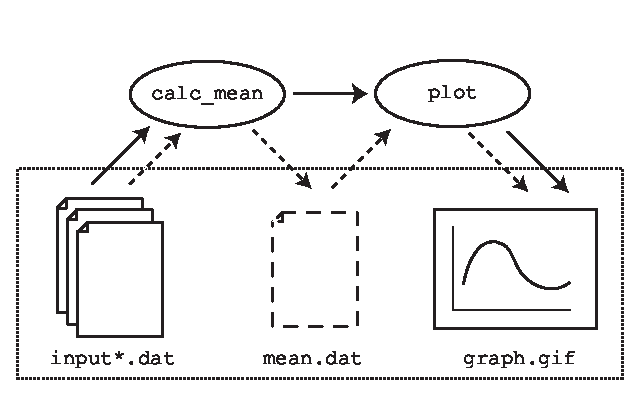
\includegraphics[height=5cm]{datapassing.eps}
\end{center}
\caption{CHANGE TO BLACK AND WHITE. Illustration of direct data passing between Styx Grid Services.  The yellow ellipses are Styx Grid Services and the dashed box contains files that exist on the client's machine.  The red arrows represent data transfers that result from the workflow in the first script in section~\ref{sec:shellscripts}.  The intermediate file {\tt mean.dat} is not required by the client and so the workflow can be arranged (second script in section~\ref{sec:shellscripts}) so that this file is passed directly between the SGSs (black arrows).}\label{fig:datapassing}
\end{figure}

%\begin{wrapfigure}{r}{50mm}
%\centering
%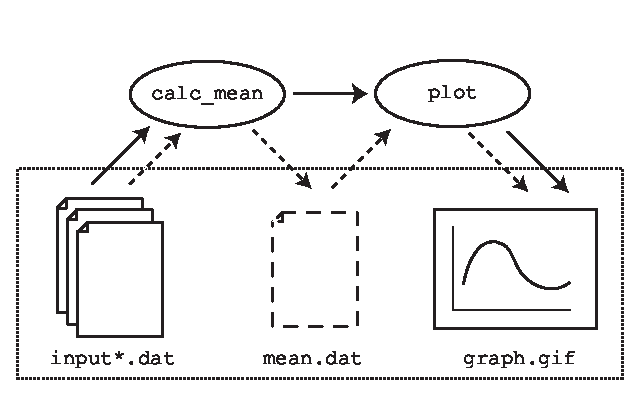
\includegraphics[width=5cm]{datapassing.eps}
%\caption{Direct data passing between Styx Grid Services}\label{fig:datapassing}
%\end{wrapfigure}



\subsubsection{Data streaming using the pipe operator.}\label{sec:pipes}
Let us imagine that the {\tt calc\_mean} program outputs data on its standard output, instead of to an output file.  Similarly, imagine that the {\tt plot} program reads data on its standard input and outputs the picture on its standard output.  The command required to execute this simple workflow (with both local programs {\em and\/} Styx Grid Services) is:

\begin{verbatim}
calc_mean input*.dat | plot > graph.gif
\end{verbatim}

Here, the intermediate data is being streamed to the local client, then streamed back out to the {\tt plot} service.  Again, we can ensure that the intermediate data are streamed directly between the services with a minor change to the command:

\begin{verbatim}
calc_mean input*.dat --sgs-ref-stdout | plot > graph.gif
\end{verbatim}

The {\tt --sgs-ref-stdout} flag is a signal to send a reference (URL) to the standard output of the {\tt calc\_mean} service to the standard input of the {\tt plot} service.  In this way the intermediate data are streamed directly between the services, across the Internet.

\subsection{Using graphical workflow tools}\label{subsec:graphical-workflow}
The command line scripting interface to the SGS system that is described above is perhaps the simplest way of creating SGS workflows.  In some cases, however, there are significant advantages in using more sophisticated graphical tools to interact with services and create workflows.  In particular, graphical interfaces can provide richer interactivity with the SGS server: progress and status can be monitored graphically, input parameters can be set using graphical controls and the service can be steered~\cite{blower:2005}.  Some users prefer to use graphical tools rather than create their own scripts.

The Taverna workbench ({\tt http://taverna.sf.net}) is a graphical workflow system that was designed for performing {\it in silico} experiments in the field of bioinformatics, but it is sufficiently general to be useful to other communities.  Using Taverna, the user can build workflows from diverse service types, including Web Services and Styx Grid Services.  EMPHASIZE WHAT WE'VE DONE!

The Triana workflow system ({\tt http://trianacode.org}) is a graphical workflow environment that can interface with many different service types (including Web Services), but cannot currently interface directly with Styx Grid Services.  There are two ways in which this can be achieved:
\begin{enumerate}
	\item {\bf Brokering:} A separate Web Services server is created that accepts SOAP messages and uses the information therein to communicate with an SGS server~\cite{blower:2005}.
	\item {\bf ``SOAP over Styx'':} The Styx Grid Service itself is modified to accept SOAP messages that are written directly to it using the Styx protocol (the message is written to a special file in the SGS namespace).  The SGS describes itself using a WSDL document that is also readable via a special file.  This WSDL document defines service operations that encapsulate the messages and data to be written to the files in the SGS namespace.  So for example, to tell the SGS to read its input data from a certain URL, the client invokes the {\tt setStdin(String url)} operation that is defined in the WSDL.  Support for this is built into WSPeer~\cite{wspeer}, the Peer-to-Peer oriented Web Service framework that is used by Triana.
\end{enumerate}

\subsection{Wrapping SGSs as WS-Resources}\label{subsec:ws-resources}

The Web Services Resource Framework (WSRF) is a recent specification which addresses the need to handle resources (WS-Resources) that maintain state across service invocations.  SGSs fit naturally into this class of entity because they maintain state that can be retrieved and modified.  WSPeer is capable of wrapping an SGS as a WS-Resource.

The process of exposing an SGS as a WS-Resource involves transforming the SGS's configuration information (Sect.~\ref{sec:wrapping}) into {\em ResourceProperties\/}, which are QName/value pairs of a specified data type that are used to describe a WS-Resource in WSDL.  Styx Grid Services define certain properties which map directly onto WSRF specifications.  An example of this is the {\tt time/} directory in the SGS namespace, which houses files containing data pertinent to the lifetime of the service.  These can be mapped directly onto the properties defined in the WS-ResourceLifetime~\cite{wsrf-lifetime} specification.  Similarly, the {\tt serviceData/} directory of the SGS namespace contains state data; clients can subscribe to receive notifications of changes to these data.  These can be exposed as WS-Notification~\cite{wsrf-notification} topics.  The ability of WSPeer to use the Styx protocol allows clients that are behind firewalls and NAT systems to receive these messages (see Sect.~\ref{sec:styx-firewalls} above).

WSPeer can expose Styx Grid Services as WS-Resources in two ways.  The first way (brokering) is to create a WSRF server that receives SOAP messages over HTTP and translates the information therein into Styx messages, which it sends to a separate SGS server.  The second is to use the Styx protocol itself to send and receive XML, as described in Section~\ref{subsec:graphical-workflow}.


\section{Conclusions}
We have introduced a new type of Internet service, the Styx Grid Service (SGS).  SGSs wrap command-line programs and allow them to be run from anywhere on the Internet, exactly as if they were local programs.  SGSs can be combined into workflows using simple shell scripts or more sophisticated graphical workflow engines.  Data can be streamed directly between SGS instances, allowing workflows to be maximally efficient.  We have shown that Styx Grid Services can operate as part of a Web Services or WSRF system through the use of methods including broker services.

A key strength of the SGS system is that it is very easy to create and use services: it is well within the reach of most end-users (scientists) to do so with no help from dedicated technical staff.  Problems connected with firewalls and NAT routers are vastly reduced compared with other systems, allowing for easy deployment and use.
%

\section*{Acknowledgements}
The authors would like to thank Tom Oinn for incorporating the SGS framework into Taverna and Vita Nuova Holdings Ltd.\ for technical help with the Styx protocol.  This work was supported by EPSRC and NERC, grant ref. GR/S27160/1.

%
% ---- Bibliography ----
%
\bibliographystyle{splncs}
\bibliography{refs}

\end{document}
